\subsubsection*{S3: component effects as complexity increases}
\begin{figure}[!htbp]
\centering
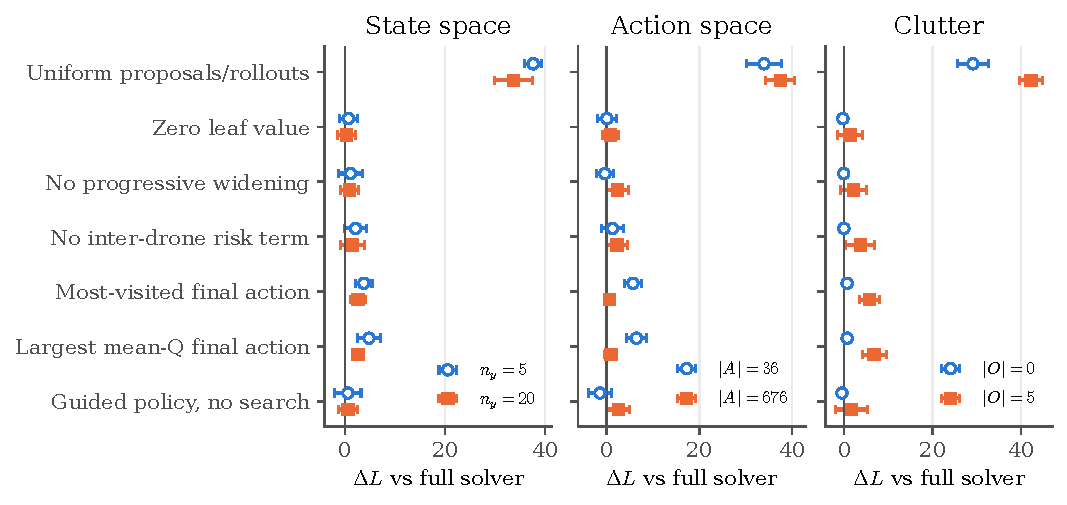
\includegraphics[width=\linewidth]{figures/component_effects.pdf}
\caption{Paired change in $L$ after removing a component at low/high factor
levels (open/filled markers); 95\% seed-block intervals.
Positive values favour the full solver.}
\end{figure}

\textbf{Guidance in expansion and rollout} has the largest measured effect.
Uniform proposals/rollouts raise $L$ by $\val{CompNoguidance}$
$\val{CompNoguidanceci}$ and change success by $\val{CompNoguidanceP}$\,pp.
The loss grows from $\val{CompNoguidanceClo}$ without obstacles to
$\val{CompNoguidanceChi}$ with five; the clutter interaction excludes zero
($\val{CompNoguidanceCint}$), whereas its state/action interactions do not.
This ablation removes both route guidance and admissible-target filtering.

\textbf{Root choice} also matters: most-visited selection raises $L$ by
$\val{CompVisitschoice}$ $\val{CompVisitschoiceci}$, and executing the
largest-mean-$Q$ action raises it by $\val{CompMaxq}$ $\val{CompMaxqci}$.
Both increases are larger with clutter (interaction intervals
$\val{CompVisitschoiceCint}$ and $\val{CompMaxqCint}$) and smaller with richer
commands ($\val{CompVisitschoiceAint}$ and $\val{CompMaxqAint}$). These
comparisons support the chosen switching rule on these tasks; they do not
make its estimated margin a calibrated confidence bound.

\textbf{Widening and the leaf value} have no statistically resolved effects
across these corners ($\val{CompNowidening}$ $\val{CompNowideningci}$ and
$\val{CompNoleaf}$ $\val{CompNoleafci}$; full estimates in
Appendix~\ref{app:components}). Routes are roughly eleven steps, comparable
to the sampled tree depth plus eight-step rollout, which may limit the leaf
value's contribution. \textbf{The inter-drone risk term} does matter:
removing it raises $L$ by $\val{CompNorisk}$ $\val{CompNoriskci}$ and changes
success by $\val{CompNoriskP}$\,pp, mostly with clutter (interaction
$\val{CompNoriskCint}$).

\textbf{Search versus its base policy.}
Removing search changes $L$ by $\val{CompHeuristic}$ $\val{CompHeuristicci}$
overall, but its action interaction is resolved ($\val{CompHeuristicAint}$):
removing search raises $L$ with 26 commands ($\val{CompHeuristicAhi}$),
while the change with 6 commands is unresolved ($\val{CompHeuristicAlo}$).
In the regression and generated suites, search rescues
$\val{BaseMultiRescued}$ multi-drone episodes and loses $\val{BaseMultiLost}$
and removing it changes $L$ by $\val{BaseMultiDL}$
$\val{BaseMultiDLci}$ (Appendix~\ref{app:regression}). With value guidance,
search has no consistent completion benefit across the evaluated suites;
the measured performance is largely explained by the guided base policy.
